\section{Methods}
\label{sec:methods}

In this manuscript, we are primarily concerned with $k$-nearest neighbors in a finite-dimensional 
vector space. Given a dataset $\textbf{X} = \{x_1 \dots x_n\}$, we define a \emph{point} or \emph{datum} $x_i \in \textbf{X}$ as a singular observation (e.g., the genome of 
an organism, the vector representation of a single image, or any entity on which we can define a \emph{distance function}).

We define a \emph{distance function} $f : \textbf{X} \times \textbf{X} \mapsto \mathbb{R}^+ \cup \{0\}$ as a function which, 
given two points $x, y \in \textbf{X}$, deterministically returns a non-negative real number. We require that the distance function 
be symmetric (i.e., $f(x, y) = f(y, x)$ for all $x, y \in \textbf{X}$) and that the distance between two points $x$ and $y$ be zero if and only if $x = y$. 
When, in addition to these constraints, the distance function obeys
the triangle inequality, it is a \emph{distance metric}, and in such cases we can guarantee that our search algorithms have perfect recall. 
Choice of distance function varies by type of data. For example, with electromagnetic spectra, we use both 
Euclidean (L2) and Cosine distances. With biological or string data, Hamming and Levenshtein distances are more appropriate.


Some of our algorithms for $\rho$- and $k$-nearest neighbors search rely on the \emph{local fractal dimension} at some point 
and length scale in the dataset, 
which we define as: 
\begin{equation} \frac{\text{log}(\frac{|B_X(q, r_1)|}{|B_X(q, r_2)|})}{\text{log}(\frac{r_1}{r_2}) } \label{1} \end{equation}
where $B_X(q, r)$ is the set of points contained in a ball of radius $r$ 
centered at a point $q$ in the dataset $\textbf{X}$; in this example, we compute fractal dimension for some radius $r_1$ and a smaller radius $r_2 = \frac{r_1}{2}$.
We stress that this concept differs from the \emph{embedding dimension} of a dataset. To illustrate the difference,
consider SDSS's APOGEE dataset, wherein each datum is a nonnegative real-valued vector of length 8,575. Hence, the \emph{embedding dimension} of this dataset is 8,575. 
However, due to physical constraints (namely, the laws that govern stellar fusion and spectral emission lines), the data are constrained to a lower-dimensional 
manifold within the 8,575-dimensional embedding space. The \emph{local fractal dimension} is an approximation of the dimensionality of that lower-dimensional manifold at a given point, for some length scale.
The notion that high-dimensional data collected from constrained generating phenomena typically only occupy a low-dimensional manifold within their embedding space is known as the \emph{manifold hypothesis}~\cite{fefferman2016testing}.


Figures 2 and 3 in~\cite{ishaq2019clustered} illustrate the low fractal dimensions of two datasets used with $\rho$-NN search in CHESS. 
We observe that for both APOGEE (Figure 2 in~\cite{ishaq2019clustered}) and GreenGenes (Figure 3 in~\cite{ishaq2019clustered}), other than the most extreme 10\% of clusters, virtually all clusters have a local fractal dimension of less than $2 \ll 8,575$
and $2 \ll 2,250$ respectively.
This suggests that APOGEE and GreenGenes are good datasets for use with entropy-scaling search algorithms like CHESS and CAKES.

We define a \emph{cluster} as a set of points with a \emph{center}, a \emph{radius}, and an approximation of the \emph{local fractal dimension}.
The \emph{center} is the geometric median of a sample of points in the \emph{cluster}, and so it is a real data point. The \emph{radius} is the
maximum distance from a point in the cluster to its \emph{center}. We estimate \emph{local fractal dimension} at the cluster radius and half
the cluster radius. Each cluster (unless it is a leaf cluster) has two child clusters in much the same way that a node in
a binary tree has two child nodes. We define the \emph{metric entropy} $\mathcal{N}_{\hat{r_c}}(D)$ of a data set $D$ under a hierarchical clustering scheme as a refinement of [7], where
metric entropy for a given cluster radius $r_c$ was the number of clusters of radius $r_c$ needed to cover all data. Here, we use a hierarchical, divisive clustering 
approach, but with early stopping criteria; clusters which satisfy a user-specified stopping criterion (e.g. a specified cardinality or radius) are not further split. 
Since we frame the asymptotic complexity of $\rho$-NN search in terms of the number of leaf clusters, the \emph{metric entropy} is best thought of in terms of the number of
leaf clusters. 


With these concepts defined, we can now pose the $k$- and $\rho$- nearest neighbors search problems.
Given a query $q$, along with a distance function $f$ defined on a dataset $\textbf{X}$, $k$-nearest neighbors search aims to find 
the set $S_q$ such that  $|S_q| = k$ and $\forall x \in \textbf{X} \setminus S_q$, $f(x, q) \leq \max\{f(y, q): y \in S_q \}$; that is,
for a given $k$, find the $k$ closest points to $q$ in $ \textbf{X}$.
We also have the $\rho$-nearest neighbors search problem, which aims to find the set $\{x \in \textbf{X}: f(q, x) \leq \rho \}$; that is, 
find all points in $\textbf{X}$ that are at most a distance $\rho$ from $q$.

Given a Cluster $C$, let $c$ be its center and $r$ be its radius. Our $\rho$- and $k$-NN algorithms make use of the following cluster 
properties:
\begin{itemize}
    \item $\delta = f(q, c)$ is the distance from the query to the cluster center $c$.
    \item $\delta_{max} = \delta + r$ is the distance from the query to the theoretically farthest possible instance in $C$.
    \item $\delta_{min} = \text{max}(0, \delta - r)$ is the distance from the query to the theoretically closest possible instance in $C$.
\end{itemize}


We define \emph{singletons} as clusters which either contain a single point (i.e., have cardinality 1) or which contain 
many instances of the same point (i.e., have cardinality greater than 1 but contain only one unique point). Singletons clearly 
have zero radius, and so $\delta_{max}  = \delta = \delta_{min}$ for these clusters. Hence, we sometimes overload the above 
notation to refer to distance from a query to a point; in these cases, we also have that $\delta_{max} = \delta = \delta_{min}$.


\subsection{Clustering}
\label{subsec:methods:clustering}

We start by building a divisive hierarchical clustering of the dataset with CLAM, using a 
similar recursive procedure as outlined in CHESS, but with the following 
improvements: better selection of poles for partitioning and depth-first dataset reordering 
(see Section ~\ref{subsubsec:methods:dataset-depth-first-reordering}). 


CLAM assumes the manifold hypothesis. 
In other words, we assume that the dataset is embedded in a $D$-dimensional space, but that the data only occupy 
a $d$-dimensional manifold, where $d \ll D$. 
While we sometimes use Euclidean notions, such as voids and volumes, to talk about geometric and topological 
properties of clusters and of the manifold, CLAM does not rely on such notions; 
they serve merely as a convenient, more intuitive way to talk about the underlying mathematics.

\subsubsection {Cluster Partitioning}

For a cluster $C$ with $|C|$ points, we begin by computing a 
random sample of $\sqrt{|C|}$ of its points, and computing pairwise distances 
between all points in the sample. Based on those pairwise distances, we compute the \emph{geometric median} of this sample; 
that is, the point which minimizes the sum of distances to all other points in the sample. This geometric median 
is $C$'s \emph{center}. The \emph{radius} of $C$ is the maximum distance from any point in $C$ to its center.
The point $l$ which is responsible for that radius (i.e., the furthest point from the center) is designated the \emph{left pole}, and the point $r$ which is furthest
from $l$ is designated the \emph{right pole}. We then partition the cluster into a \emph{left child} and \emph{right child}, where the 
left child contains all points in the cluster which are closer to $l$ than to $r$, and the right child contains all 
points in the cluster which are closer to $r$ than to $l$. Without loss of generality, we assign to the left child 
those points which are equidistant from $l$ and $r$. Starting from a root-cluster containing the entire dataset, we 
repeat this procedure until each leaf contains only one datum or some other user-specified stopping criterion 
is met. 

This process is described in Algorithm \ref{alg:partition}.


\begin{algorithm} % enter the algorithm environment
\caption{ClusterPartition(\emph{C})} % give the algorithm a caption
\label{alg:partition} % and a label for \ref{} commands later in the document
\begin{algorithmic} % enter the algorithmic environment
    \STATE $m \Leftarrow \lfloor \sqrt{|C|} \rfloor$
    \STATE $seeds \Leftarrow m$ random points from $C.points$
    \STATE $c \Leftarrow$ geometric median of $seeds$
    \STATE $l \Leftarrow \argmax d(c,x) \ \forall \ x \in C.points$
    \STATE $r \Leftarrow \argmax d(l,x) \ \forall \ x \in C.points$
    \STATE $left \Leftarrow \{x | x \in C.points \land d(l,x) \le d(r,x)\}$
    \STATE $right \Leftarrow \{x | x \in C.points \land d(r,x) < d(l,x)\}$
    \IF{$|left| > 1$}
        \STATE ClusterPartition($left$)
    \ENDIF
    \IF{$|right| > 1$}
        \STATE ClusterPartition($right$)
    \ENDIF
\end{algorithmic}
\end{algorithm}

\subsubsection {Dataset Depth-First Reordering}
\label{subsubsec:methods:dataset-depth-first-reordering}

CAKES also improves upon CHESS by reordering the dataset. In CHESS, each cluster stored a list of indices into the dataset, 
which we used during search to retrieve a cluster's points. 
Though this approach allowed us to retrieve the points in constant 
time, its memory cost was prohibitively high; since each cluster stores indices for each of its
points, for a dataset with cardinality $n$, we store a total of $n$ indices at each depth in the tree.
With $\log{}n$ levels in the tree, this approach had $\mathcal{O}(n\log{}n)$ memory cost. 


One may think to improve this memory cost to $\mathcal{O}(n)$ by storing only the indices of points at 
the leaf cluster level.
This approach, however, introduces an $\mathcal{O}(n)$ time cost whenever we need to find the indices for 
a non-leaf cluster, since it requires a traversal of the subtree rooted at that cluster.


In this work, we introduce a new approach, wherein after building the cluster tree, we reorder the dataset 
so that points are stored in a depth-first order. Then, within each cluster, we need only 
store the cluster's cardinality and an \emph{offset} to access the cluster's points from the dataset. Each parent cluster 
have the same offset as its left child, and each right child has an offset equal to their sibling's offset
plus their siblings's cardinality. With no additional memory cost nor time cost for retrieving points during search, 
dataset depth-first reordering offers significant improvements over the approach used in CHESS.


\subsubsection {Scaling Behavior of Cluster Radii}
\label{subsubsec:methods:guaranteed-decrease-in-cluster-radii}
While it may be tempting to assume that cluster radii decrease with each application of Cluster Partition (refer to Algorithm \ref{alg:partition}), unfortunately, this assumption is incorrect. 
Fortunately, we \emph{can} make some guarantees about the scaling behavior of cluster radii; in particular, we prove in this section that cluster radii will stop increasing after at most 
$d$ partitions, where $d$ is the dimensionality of the dataset. 

We can describe a $d$-dimensional distribution of data by choosing some set of $d$ mutually orthogonal axes.
Let $2R$ be the maximum pairwise distance among the points in the dataset. 
We choose the axes such that the two points that are $2R$ apart lie \emph{along one of the axes}. 
Thus, a $d$-dimensional hyper-sphere of radius $R$ would bound the dataset. 
In the worst case, (i.e., with a uniform-density distribution that fills the $d$-sphere), our axes will be such that $2R$ is the maximum pairwise distance along every axis. 
Such a distribution would also produce a balanced clustering.


In this case, Cluster Partition will select a maximally distant pair of points to use as poles, i.e., it will choose one of the $d$ axes along
which to split the cluster into two children. 
After one application of Algorithm \ref{alg:partition}, the maximum pairwise distance along that axis will be
bounded above by $R$. 
The next recursive Cluster Partition will select another of the $d$ axes. 
Thus, after at most $d$ applications of Algorithm \ref{alg:partition}, the
maximum pairwise distance along each axis will be bounded above by $R$. 
The overall (i.e., not restricted to one axis) maximum pairwise distance 
will be bounded above by $R\sqrt{2}$ by, for example, two instances that lie at the extrema of different axes. 

Thus, starting with a cluster $C$ of radius $R$, after at most $d$ Partitions, the descendants of $C$ will each have radius
bounded above by $\frac{R}{\sqrt{2}}$. In other words, cluster radii are guaranteed to decrease by a multiplicative factor of $\frac{\sqrt{2}}{2}$ after at 
most $d$ applications of Algorithm \ref{alg:partition}. 


Note that, in practice, we never see a balanced clustering. Cluster Partition  produces unbalanced trees due to the varying density of the sampling 
in different regions of the manifold and the low dimensional "shape" of the manifold. Further, the cluster radii decrease by a factor much larger than 
$\frac{\sqrt{2}}{2}$ in practice, and the upper bound of $d$ partitions is seldom realized. 


\begin{figure}[ht!]
    \centering
    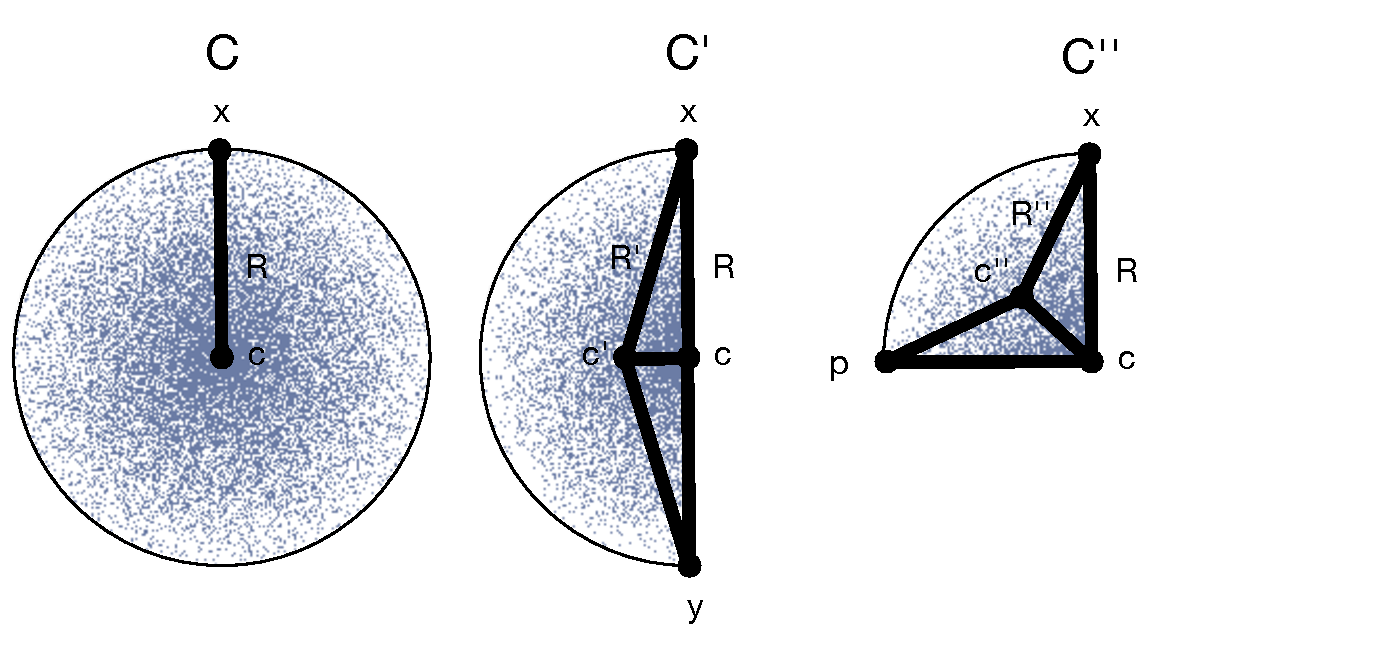
\includegraphics[width=3.4in]{images/geometry/geometry.pdf}
    \caption{Scaling Behavior of Radii in a Two-Dimensional Uniform-Density Disk. $R$ 
    denotes the radius of the root cluster $C$, and $o$ denotes its center. The right 
    triangle formed by $o$, $o'$, and $y+$ in $C'$ shows that $R \leq R'$, where $R'$ is the radius of $C'$.
    Hence, the radius of a child cluster can be larger than its parent. $C''$ 
    illustrates that after we have consumed all $d$ axes, the radius of a child cluster
    is bounded above by $\frac{R}{\sqrt{2}}$.}
    \label{fig:methods:scaling_behavior}
\end{figure}

\subsubsection {Complexity}
\label{subsubsec:methods:clustering:complexity}

The asympotitic complexity of Partition is the same as described in~\cite{ishaq2019clustered}
By using an approximate partitioning with a $\sqrt{n}$ sample, we achieve $\mathcal{O}(n)$ cost of 
partitioning and $\mathcal{O}(n \log n)$ cost of building the tree. This is a significant improvement over 
exact partitioning and tree-building, which have $\mathcal{O}(n^2)$ and $\mathcal{O}(n^2 \log n)$ costs respectively.


\subsection {Index-Building and Sharded Search}
\label{subsec:methods:index-building}
In this work, we also introduce the method of \emph{sharding} for $k$-nearest neighbors search.
With this approach, we aim to leverage the fact that $\rho$-nearest neighbors search is typically 
much faster than $k$-nearest neighbors search. 


We begin by randomly partitioning the dataset into $s$ shards, where $s$ is determined based 
on some naive auto-tuning. On the first shard, we perform 
$k$-nearest neighbors search using one of the four algorithms described in Section~\ref{subsec:methods:knn-search}.
The result of this search will give us the $k$ closest neighbors to the query \emph{in the first shard}. We then take the furthest of 
those $k$ neighbors and use its distance from the query as the radius for use with $\rho$-nearest neighbors search (see Section~\ref{subsec:methods:rnn-search}) 
on each remaining shard. We then take the union of the results of these $\rho$-nearest neighbors searches, along with the $k$ neighbors
from the first shard, and then linear search over those points to find the actual $k$ nearest neighbors.


Note that the size of the shards is not necessarily consistent; it is often optimal to have the first shard be smaller than the others,
since the first shard is the only one for which we perform $k$-nearest neighbors search. However, making this first shard too small
introduces the risk of significantly overestimating the radius, resulting in much slower $\rho$-nearest neighbors search on the subsequent shards.
Finding the precise optimal ratio between the size of the first shard and the size of the remaining shards, as well 
as computing the expected level of error between the distance from the $k$-th closest neighbor in the first shard and the 
actual $k$-th closest neighbor, are topics for future work.

\subsection{\texorpdfstring{$\rho$}{p}-Nearest Neighbors Search}
\label{subsec:methods:rnn-search}

We conduct $\rho$-nearest neighbors search as described in \cite{ishaq2019clustered}, but 
with the following improvement: when a cluster overlaps with the query ball, instead of  
always proceeding with both of its children, we proceed only with those children which 
also overlap with the query ball. This improvement is demonstrated in Algorithm \ref{alg:rnn}.

\begin{algorithm} 
    \caption{$\rho$-NN(\emph{clusters, query, r})} 
    \label{alg:rnn} 
    \begin{algorithmic}
        \REQUIRE $r \geq 0$
        \REQUIRE $clusters \neq \emptyset$
        \STATE $results \Leftarrow \emptyset$
        \IF{$clusters.left \land clusters.left \cap B_X(query, r) \neq \emptyset$}
            \IF{$clusters.left.\delta$ $\leq$ $r$ + $clusters.left.radius$}
                \STATE $\rho$-NN($clusters.left, query, r$)
            \ENDIF
        \ENDIF
        \IF{$clusters.right \land clusters.right \cap B_X(query, r) \neq \emptyset$}
            \IF{$clusters.right.\delta$ $\leq$ $r$ + $clusters.right.radius$} 
                \STATE $\rho$-NN($clusters.right, query, r$)
            \ENDIF
        \ENDIF
        \IF{$\neg$$clusters.left$ $\land \neg$$clusters.right$}
            \FOR{$p \in clusters.points$}
                \IF{$p.\delta \leq r$}
                    \STATE $results.push((p, r))$
                \ENDIF
            \ENDFOR
        \ENDIF
        \STATE Return $results$
    \end{algorithmic}
    \end{algorithm}


The asymptotic complexity of $\rho$-nearest neighbors is the same as in ~\cite{ishaq2019clustered}, namely:

\begin{gather}
    \mathcal{O}\Bigg(
    \underbrace{\log_2 \mathcal{N}_{\hat{r_c}}(D)}_{\textrm{metric entropy}} +
    \overbrace{\left|B_D(q,r)\right|}^{\textrm{output size}}
    \underbrace{\left(\frac{r+2\hat{r_c}}{r}\right)^d}_{\textrm{scaling factor}}
     \Bigg)
     \label{hierarchical-complexity}
\end{gather}

where $\hat{r_c}$ is the \textit{mean} cluster radius of leaf clusters, $\mathcal{N}_{\hat{r_c}}(D)$ is the metric entropy at that radius, $B_D(q,r)$ is a ball of data points around the query $q$ at search radius $r$, and $d$ is the factal dimension around the query in a region of radius $r$.

\subsection{\texorpdfstring{$k$}{k}-Nearest Neighbors Search}
\label{subsec:methods:knn-search}

In this section, we present four novel algorithms for exact $k$-nearest neighbors search: $k$-NN by Repeated $\rho$-NN, Sieve Search, Sieve Search with Separate Centers, 
and Greedy Sieve. 
We use a preliminary auto-tuning function to predict the variant and shard size (see Section~\ref{subsec:methods:index-building}) which will perform 
best for a given query, dataset, and value of $k$. We then proceed with search using that variant on the first shard. 

In these algorithms, we typically use $H$, for \emph{hits}, to refer to the data structure which stores the closest points to the query found so far and
$Q$ to refer to the data structure which stores the clusters (and, for Sieve and Sieve with Centers, points) which are still in contention for being one of the nearest neighbors.


\subsubsection{$k$-NN by Repeated $\rho$-NN}
\label{subsubsec:methods:knn-search:repeated-rnn}


In this algorithm, we perform $\rho$-nearest neighbors search small search radius, repeatedly increasing the radius until $k$ neighbors
have been found.

Let $H$ be the set of nearest neighbors found thus far.
Search starts with a radius $m$ equal to the radius of the root cluster divided by
the cardinality of the dataset. We perform $\rho$-NN search with radius $m$. 
If no points are within a distance $m$ of the query, we increase the radius by a factor of arg
2 and perform $\rho$-NN search again, repeating until at least one point is found, i.e., 
until $|H| > 0$.


Once $|H| > 0$, we continue to perform $\rho$-NN search, but instead of 
increasing the radius by a factor of 2 on each iteration, we increase it by a factor determined 
by the local fractal dimension in the region of the dataset around the query ball. 
In particular, 
we increase the radius by a factor of 
\begin{equation} \argmin \left(2, \left({\frac{k}{|H|}}\right)^{\frac{1}{\mu}}\right) \label{2} \end{equation}
where $\mu$ is the harmonic mean of the local fractal dimensions (abbreviated lfd in algorithm below) of 
each cluster which contains one of the nearest neighbors found thus far. We use the harmonic mean to 
ensure that $\mu$ is not dominated by outlier clusters with very high fractal dimension. 
Intuitively, the factor by which we increase the radius should be \emph{inversely} related to the number of points found so far. 
Additionally, when the local fractal dimension at the radius scale from the previous iteration is low, this suggests that the data 
are relatively concentrated in that region; in other words, a small increase in the radius would likely encounter unoccupied space around the manifold, so a larger radius increase is needed. Thus, in this case, the factor of radius increase should be \emph{directly} related to the 
local fractal dimension. Once $|H| >= k$, we return the $k$ closest points.

\begin{algorithm} % enter the algorithm environment
    \caption{Repeated$\rho$-NN(\emph{root, query, k})} % give the algorithm a caption
    \label{alg:knn-by-rnn} % and a label for \ref{} commands later in the document
    \begin{algorithmic} % enter the algorithmic environment
        \STATE $H \Leftarrow$ $\emptyset$
        \STATE $m \Leftarrow$ $\frac{root.radius}{|root|}$
        \WHILE {$|H| = 0$}
            \STATE $H.push(\rho$-NN$(root, query, m)$)
            \STATE $m \Leftarrow 2m$
        \ENDWHILE
        \WHILE {$|H| < k$}
            \STATE $Q \Leftarrow \{ C: \exists p \in H \land p \in C \}$
            \STATE $\mu \Leftarrow |Q| \sum_{C \in Q} \frac{1}{C.lfd} $
            \STATE $m \Leftarrow \argmin \left(2, \left({\frac{k}{|H|}}\right)^{\frac{1}{\mu}}\right)$
            \STATE $H.push(\rho$-NN$(root, query, m)$)
        \ENDWHILE
        \STATE $H.sort()$
        \STATE Return $H[0], H[1], \cdots H[k-1]$
    \end{algorithmic}
    \end{algorithm}

\subsubsection{Complexity of $k$-NN by Repeated $\rho$-NN Search}
\label{paragraph:methods:repeated-rnn-complexity}

Our complexity bounds for $k$-NN by Repeated $\rho$-NN rely on the assumption that the query point is sampled from the same distribution
(i.e. arises from the same generating phenomenon) as the rest of the data. From this assumption, we can infer that the local fractal dimension
at the query point is not significantly different from the mean local fractal dimension of clusters nearby the query.

We find it useful to adopt the terminology used in 
\cite{ishaq2019clustered} and \cite{yu2015entropy} and address \emph{coarse search} and \emph{fine search} separately. 
Coarse search refers to the process of identifying clusters
which have overlap with the query ball (i.e., which are likely to contain one of the $k$ nearest neighbors). 
Fine search refers to the process
of identifying the $k$ nearest neighbors among the points in those clusters identified by coarse search.

In ~\cite{ishaq2019clustered}, we claimed that the complexity of coarse search for $\rho$-NN is $\mathcal{O}(\log{2}$\mathcal{N}_{\hat{r_c}}(D)$)$, 
where $m$\mathcal{N}_{\hat{r_c}}(D)$$ is the metric entropy of the dataset $D$. 
To adjust this bound for $k$-NN by Repeated $\rho$-NN, we must estimate the number of iterations 
of $\rho$-NN needed to find at least $k$ neighbors. 
    

Based on the assumption that the local fractal dimension at the query point is not significantly different than that of 
nearby clusters, the factor from Equation \ref{2} suggests that in the expected case, we need only two iterations of 
$\rho$-NN to find $k$ neighbors: one iteration to find at least one neighbor, and the one more to find enough remaining neighbors.
Since this is a constant factor, it does not affect the asymptotic complexity of coarse search, and thus we have that 
the complexity of coarse search for $k$-NN by Repeated $\rho$-NN is $\mathcal{O}(\log_2{m})$.

To determine the asymptotic complexity of fine search, we must estimate $|F|$, the 
number of clusters for which we must look at all of the cluster's points. With $\rho$-NN 
search, $F$ is the union of clusters which are within a distance of $r + r_c$ from the query,
where $r$ is the search radius and $r_c$ is the radius of leaf clusters,
as in \cite{yu2015entropy}. With $k$-NN by Repeated $\rho$-NN, however, 
the value of $r$ is dependent on the distance to the $k$th nearest neighbor, which 
is query-dependent. Thus, for $k$-NN by Repeated $\rho$-NN, we adjust the definition of 
$F$ to be the union of clusters which are within a distance of $r' + r_c$ from the query, 
where $r'$ is the distance to the $k$th nearest neighbor and $r_c$ is defined as before.

~\cite{yu2015entropy} showed that $|F| \leq \gamma |B(q, r')|\left(\frac{r'+ 2r_c}{r'}\right)^d$, where $\gamma$ is a constant. 
By definition of 
$r'$, we have that $|B(q, r')| = k$. Thus, we have that $|F| \leq \gamma k\left(\frac{r'+ 2r_c}{r'}\right)^d$. 

    
It remains to provide an estimate for $r'$. 
To do this, we once again rely on the assumption that the query is from the same distribution as the rest of the data, 
and thus the local fractal dimension at the query point is not significantly different than that of nearby clusters.


We let $d_i$ be the local fractal dimension of some cluster $C_i$ near the query point (i.e., some cluster identified during coarse search).
While ordinarily we compute local fractal dimension 
by comparing cardinalities of two balls centered at \emph{the same} point at two different radii, in order to estimate $r'$, 
we instead compare the cardinality of a ball \emph{around the query} of radius $r'$ to the cardinality \emph{of cluster $C_i$} at its radius $r_i$.
We justify this approach by noting that, since the query is from the same distribution as the rest of the data, we could "drag" the query to 
the center of $C_i$ without significantly changing the local fractal dimension at the query point. 


By ~\ref{2}, we then have that \begin{equation} d_i = \frac{\log{}\frac{|C_i|}{k}}{\log{}\frac{r_i}{r'}}. \label{4} \end{equation}

Since $d_i$, $|C_i|$, $r_i$, and $k$ are all known values, we can solve equation ~\ref{4} for $r'$ to get
\begin{equation} r' = r_i\left(\frac{k}{|C_i|}\right)^{\frac{1}{d_i}}. \label{5} \end{equation}
    
Putting our bounds for coarse and fine search together, we have that $k$-NN by Repeated $\rho$-NN has 
$\mathcal{O}\left(\log_2{\mathcal{N}_{\hat{r_c}}(D)} + k\left(\frac{r_i\left(\frac{k}{|C_i|}\right)^{\frac{1}{d_i}}+ 2r_c}{r_i\left(\frac{k}{|C_i|}\right)^{\frac{1}{d_i}}}\right)^d\right)$ 
time complexity, where $\mathcal{N}_{\hat{r_c}}(D) is the metric entropy of the dataset, $d$ is the dimensionality of the dataset, $r_i$ is the radius of some cluster $C_i$
near the query ball, $d_i$ is the local fractal dimension of $C_i$, $r_c$ is the radius of leaf clusters, and $k$ is the number of nearest neighbors. 

\subsubsection{Sieve Search}
\label{subsubsec:methods:knn-search:sieve}
With Sieve Search, we begin by letting $Q$ be a list containing the root cluster. 
While $Q$ contains at least one cluster (i.e., $Q$ is not a list of only points), we repeat the process described in 
the following paragraphs. 

First, 
we aim to find the element $q_{\tau} \in Q$ with the smallest $\delta_{max}$ such that 
$q_{\tau}$ and all elements in $Q$ with smaller $\delta_{max}$ collectively contain at least $k$ points. 

To find this element, 
we use a process similar to the Partition algorithm used in Quicksort~\cite{10.1093/comjnl/5.1.10}, adjusted to account for the varying cardinalities of elements in $Q$. 
Our modified version of this algorithm finds the smallest index $i$ such 
that all elements in $Q$ with $\delta_{max}$ closer to or equal to $Q[i]$'s $\delta_{max}$ collectively have cardinality greater
than or equal to $k$. We consider $Q[i]$ to be our $q_{\tau}$, and our threshold 
$\tau$ to be $Q[i]$'s $\delta_{max}$.

We then remove from $Q$ any element whose $\delta_{min}$ is greater than $\tau$. Then, for each element left 
in $Q$, if it is a leaf or contains $k$ or fewer points, we remove it and all of its points to $Q$. Finally, we
replace all remaining non-leaf clusters in $Q$ with their children. 

We complete this process until $Q$ contains only points. At this point, we 
just use Algorithm 4 to find the $k$th 
nearest neighbor and return all points to the left of it. 

This process is described in Algorithm~\ref{alg:sieve}. 

\begin{algorithm} % enter the algorithm environment
    \caption{Sieve(\emph{tree, query, k})} % give the algorithm a caption
    \label{alg:sieve} % and a label for \ref{} commands later in the document
    \begin{algorithmic} % enter the algorithmic environment
        \REQUIRE $tree$, $query$, $k$
        \STATE $Q \Leftarrow$ [$tree.root$]
        \WHILE{$|Q| > k$}
            \STATE $i \Leftarrow QuicksortPartition(Q, k, 0, |Q| - 1)$
            \STATE $\tau \Leftarrow Q[i].\delta_{max}$
            \FOR {$q \in Q$}
                \IF {$q.\delta_{min} > \tau$}
                    \STATE $Q.pop(q)$
                \ENDIF
            \ENDFOR
            \FOR {$q \in Q$}
                \IF {$q.isLeaf \lor |q| \leq k$}
                    \STATE $Q.push(q.points)$
                \ELSE
                    \STATE $[l, r] \Leftarrow q.children$
                    \STATE $Q.push([l, r])$   
                \ENDIF
                \STATE $Q.pop(q)$
            \ENDFOR 
        \ENDWHILE
        \STATE Return $Q$
    \end{algorithmic}
    \end{algorithm}

\subsubsection{Sieve Search with Separate Centers}
\label{subsubsec:methods:knn-search:sieve2}
Sieve Search with Separate Centers is the same as Sieve Search, but with the following modification: clusters 
in $Q$ are represented twice-- once as their center and once as the rest of their points. 
Because we have that for any cluster $C$, $C.\delta \leq C.\delta_{max}$, representing the cluster 
center separately from the rest of the points causes the threshold $\tau$ to decrease more quickly, 
thus allowing us to eliminate some clusters from $Q$ earlier in the process. More discussion about 
when this algorithm is preferable to Sieve Search is in Section 4: Results. 


\subsubsection{Greedy Sieve}
\label{subsubsec:methods:knn-search:greedy-search}

With Greedy Sieve, we first let $Q$ be a min queue of clusters based on $\delta_{min}$. We initialize $Q$ with the root cluster.
Let $H$ be a fixed-size ($k$) max queue of points based on $\delta$. This queue starts empty.

While $H$ has fewer than $k$ clusters or $\delta$ of the top priority element in $H$ is greater 
than $\delta_{min}$ of the top priority element in $Q$, we do the following:
\begin{enumerate}
\item While the top priority element $q$ in $Q$ is not a leaf, pop $q$ from $Q$ and push its children.
\item For each point $p \in q$, push $p$ to $H$. 
\item Pop from $H$ until $H$ has $k$ points. 
\end{enumerate}
After this process, the points left in $H$ are the $k$ nearest neighbors of $q$. 

This process is described in Algorithm \ref{alg:greedy_search}.

\begin{algorithm} 
\caption{GreedySearch(\emph{root, query, k})} 
\label{alg:greedy_search} 
\begin{algorithmic}
    \STATE $Q \Leftarrow$ priority queue
    \STATE $Q.push(root)$
    \STATE $H \Leftarrow$ priority queue
    \WHILE{$|H| < k \lor H.pop.\delta > Q.pop.\delta_{min}$}
        \WHILE{$\neg Q.pop.isLeaf$}
            \STATE $[l, r] \Leftarrow Q.pop().children$
            \STATE $Q.push([l, r])$
        \ENDWHILE
        \STATE $leaf \Leftarrow Q.pop()$
        \STATE $H.push(leaf)$
        \WHILE{$|H| > k$}
            \STATE $H.pop()$
        \ENDWHILE
    \ENDWHILE
    \STATE Return $H$
\end{algorithmic}
\end{algorithm}

\subsubsection{Complexity of Sieve Algorithms}
\label{paragraph:methods:sieve-complexity}


% Our $k$-NN algorithms do not use two completely distinct phases of coarse and fine search, 
% as is the case in $\rho$-NN search. Still, this distinction is useful in analyzing 
% the asymptotic complexity of $k$-NN search. In particular, we can think of the complexity of 
% coarse search as an estimate of how many clusters we examine during search, and 
% the complexity of fine search as an estimate of how many clusters we must examine all the points 
% from during search, even if we do not actually perform these as two distinct phases. 


% To determine the asymptotic complexity of fine search, we must estimate $|F|$, the 
% number of clusters we must examine all the points from during search. With $\rho$-NN 
% search, $F$ is the union of clusters which are within a distance of $r + r_c$ from the query,
% where $r$ is the search radius and $r_c$ is the radius of leaf clusters,
% as in \cite{yu2015entropy}. With $k$-NN search, however, 
% the value of $r$ is dependent on the distance to the $k$th nearest neighbor, which 
% is query-dependent. Thus, for $k$-NN search, we  adjust the definition of 
% $F$ to be the union of clusters which are within a distance of $r' + r_c$ from the query, 
% where $r'$ is the distance to the $k$th nearest neighbor and $r_c$ is defined as before.

% By the triangle inequality, we have that $F \subseteq B(q, r' + 2r_c)$, 
% where $B(q, r' + r_c)$ is the ball of radius $r' + r_c$ centered at $q$.
% Hence, $|F| \leq |B(q, r' + 2r_c)|$.

% Now we have that \begin{align*} \mathbb{E}_q[|B(q, r' + 2r_c)|] &\leq \gamma|B(p, r' + 2r_c)| \\ %because of the assumption that density at different locations on the manifold differ by only a constant factor%
%     &\leq \gamma|B(p, r')|\left(\frac{r' + 2r_c}{r'}\right)^d \label{5}\\ %because d = lfd tells us how the number of additional hits reached scales with a change in radius, and our ratio between radii is (r' + 2r_c)/r'%
%     &\leq \gamma^2 \mathbb{E}[|B(q, r')|]\left(\frac{r'+2r_c}{r'}\right)^d \\ %using density bound again to go from a statement about an arbitrary point back to a statement about the query%
%     &\leq \gamma^2 k\left(\frac{r'+ 2r_c}{r'}\right)^d  \\   %using the fact that for k-nn, the number points in the query ball is k%
% \end{align*}

